%% FEUP THESIS STYLE for LaTeX2e
%% how to use feupteses (English version)
%%
%% FEUP, JCL & JCF, 31 July 2012
%%
%% PLEASE send improvements to jlopes at fe.up.pt and to jcf at fe.up.pt
%%

%%========================================
%% Commands: pdflatex tese
%%           bibtex tese
%%           makeindex tese (only if creating an index)
%%           pdflatex tese
%% Alternative:
%%          latexmk -pdf tese.tex
%%========================================

\documentclass[11pt,a4paper,twoside,openright]{report}

%% For iso-8859-1 (latin1), comment next line and uncomment the second line
\usepackage[utf8]{inputenc}
\usepackage{indentfirst}
%\usepackage[latin1]{inputenc}

%% English version

%% MIEIC options
\usepackage[mieic]{feupteses}
%\usepackage[mieic,juri]{feupteses}
%\usepackage[mieic,final]{feupteses}
%\usepackage[mieic,final,onpaper]{feupteses}

%% Additional options for feupteses.sty: 
%% - onpaper: links are not shown (for paper versions)
%% - backrefs: include back references from bibliography to citation place

%% Uncomment the next lines if side by side graphics used
%\usepackage[lofdepth,lotdepth]{subfig}
%\usepackage{graphicx}
%\usepackage{float}

%% Include color package
\usepackage{color}
\definecolor{cloudwhite}{cmyk}{0,0,0,0.025}

%% Include source-code listings package
\usepackage{listings}
\lstset{ %
	language=C,                        % choose the language of the code
	basicstyle=\footnotesize\ttfamily,
	keywordstyle=\bfseries,
	numbers=left,                      % where to put the line-numbers
	numberstyle=\scriptsize\texttt,    % the size of the fonts that are used for the line-numbers
	stepnumber=1,                      % the step between two line-numbers. If it's 1 each line will be numbered
	numbersep=8pt,                     % how far the line-numbers are from the code
	frame=tb,
	float=htb,
	aboveskip=8mm,
	belowskip=4mm,
	backgroundcolor=\color{cloudwhite},
	showspaces=false,                  % show spaces adding particular underscores
	showstringspaces=false,            % underline spaces within strings
	showtabs=false,                    % show tabs within strings adding particular underscores
	tabsize=2,	                    % sets default tabsize to 2 spaces
	captionpos=b,                      % sets the caption-position to bottom
	breaklines=true,                   % sets automatic line breaking
	breakatwhitespace=false,           % sets if automatic breaks should only happen at whitespace
	escapeinside={\%*}{*)},            % if you want to add a comment within your code
	morekeywords={*,var,template,new}  % if you want to add more keywords to the set
	}
	
	%% Uncomment to create an index (at the end of the document)
	%\makeindex
	
	%% Path to the figures directory
	%% TIP: use folder ``figures'' to keep all your figures
	\graphicspath{{figures/}}
	
	%%----------------------------------------
	%% TIP: if you want to define more macros, use an external file to keep them
	%some macro definitions

% format
\newcommand{\class}[1]{{\normalfont\slshape #1\/}}

% entities
\newcommand{\Feup}{Faculdade de Engenharia da Universidade do Porto}

\newcommand{\svg}{\class{SVG}}
\newcommand{\scada}{\class{SCADA}}
\newcommand{\scadadms}{\class{SCADA/DMS}}

	%%----------------------------------------
	
	%%========================================
	%% Start of document
	%%========================================
	\begin{document}
		
		%%----------------------------------------
		%% Information about the work
		%%----------------------------------------
		\title{Electronic Assessment for Software Development Certifications}
		\author{Nelson Mendes}
		
		%% Uncomment next line for date of submission
		%\thesisdate{July 31, 2008}
		
		%%Uncomment next line for copyright text if used
		%\copyrightnotice{Name of the Author, 2008}
		
		\supervisor{Supervisor}{João Pascoal Faria}
		
		%% Uncomment next line if necessary
		%\supervisor{Second Supervisor}{Name of the Supervisor}
		
		%% Uncomment committee stuff in the final version if used
		%\committeetext{Approved in oral examination by the committee:}
		%\committeemember{Chair}{Doctor Name of the President}
		%\committeemember{External Examiner}{Doctor Name of the Examiner}
		%\committeemember{Supervisor}{Doctor Name of the Supervisor}
		%\signature
		
		%% Specify cover logo (in folder ``figures'')
		\logo{uporto-feup.pdf}
		
		%% Uncomment next line for additional text  below the author's name (front page)
		%\additionalfronttext{PDIS}
		
		%%----------------------------------------
		%% Preliminary materials
		%%----------------------------------------
		
		% remove unnecssary \include{} commands
		\begin{Prolog}
			%\chapter*{Abstract}

Here goes the abstract written in English.

Lorem ipsum dolor sit amet, consectetuer adipiscing elit. Sed vehicula
lorem commodo dui. Fusce mollis feugiat elit. Cum sociis natoque
penatibus et magnis dis parturient montes, nascetur ridiculus
mus. Donec eu quam. Aenean consectetuer odio quis nisi. Fusce molestie
metus sed neque. Praesent nulla. Donec quis urna. Pellentesque
hendrerit vulputate nunc. Donec id eros et leo ullamcorper
placerat. Curabitur aliquam tellus et diam. 

Ut tortor. Morbi eget elit. Maecenas nec risus. Sed ultricies. Sed
scelerisque libero faucibus sem. Nullam molestie leo quis
tellus. Donec ipsum. Nulla lobortis purus pharetra turpis. Nulla
laoreet, arcu nec hendrerit vulputate, tortor elit eleifend turpis, et
aliquam leo metus in dolor. Praesent sed nulla. Mauris ac augue. Cras
ac orci. Etiam sed urna eget nulla sodales venenatis. Donec faucibus
ante eget dui. Nam magna. Suspendisse sollicitudin est et mi. 

Fusce sed ipsum vel velit imperdiet dictum. Sed nisi purus, dapibus
ut, iaculis ac, placerat id, purus. Integer aliquet elementum
libero. Phasellus facilisis leo eget elit. Nullam nisi magna, ornare
at, aliquet et, porta id, odio. Sed volutpat tellus consectetuer
ligula. Phasellus turpis augue, malesuada et, placerat fringilla,
ornare nec, eros. Class aptent taciti sociosqu ad litora torquent per
conubia nostra, per inceptos himenaeos. Vivamus ornare quam nec sem
mattis vulputate. Nullam porta, diam nec porta mollis, orci leo
condimentum sapien, quis venenatis mi dolor a metus. Nullam
mollis. Aenean metus massa, pellentesque sit amet, sagittis eget,
tincidunt in, arcu. Vestibulum porta laoreet tortor. Nullam mollis
elit nec justo. In nulla ligula, pellentesque sit amet, consequat sed,
faucibus id, velit. Fusce purus. Quisque sagittis urna at quam. Ut eu
lacus. Maecenas tortor nibh, ultricies nec, vestibulum varius, egestas
id, sapien. 

Phasellus ullamcorper justo id risus. Nunc in leo. Mauris auctor
lectus vitae est lacinia egestas. Nulla faucibus erat sit amet lectus
varius semper. Praesent ultrices vehicula orci. Nam at metus. Aenean
eget lorem nec purus feugiat molestie. Phasellus fringilla nulla ac
risus. Aliquam elementum aliquam velit. Aenean nunc odio, lobortis id,
dictum et, rutrum ac, ipsum. 

Ut tortor. Morbi eget elit. Maecenas nec risus. Sed ultricies. Sed
scelerisque libero faucibus sem. Nullam molestie leo quis
tellus. Donec ipsum. Nulla lobortis purus pharetra turpis. Nulla
laoreet, arcu nec hendrerit vulputate, tortor elit eleifend turpis, et
aliquam leo metus in dolor. Praesent sed nulla. Mauris ac augue. Cras
ac orci. Etiam sed urna eget nulla sodales venenatis. Donec faucibus
ante eget dui. Nam magna. Suspendisse sollicitudin est et mi. 

Phasellus ullamcorper justo id risus. Nunc in leo. Mauris auctor
lectus vitae est lacinia egestas. Nulla faucibus erat sit amet lectus
varius semper. Praesent ultrices vehicula orci. Nam at metus. Aenean
eget lorem nec purus feugiat molestie. Phasellus fringilla nulla ac
risus. Aliquam elementum aliquam velit. Aenean nunc odio, lobortis id,
dictum et, rutrum ac, ipsum. 

Ut tortor. Morbi eget elit. Maecenas nec risus. Sed ultricies. Sed
scelerisque libero faucibus sem. Nullam molestie leo quis
tellus. Donec ipsum. 

\chapter*{Resumo}

O Resumo fornece ao leitor um sumário do conteúdo da dissertação.
Deverá ser breve mas conter detalhe suficiente e, uma vez que é a porta
de entrada para a dissertação, deverá dar ao leitor uma boa impressão
inicial.

Este texto inicial da dissertação é escrito no fim e resume numa
página, sem referências externas, o tema e o contexto do trabalho, a
motivação e os objectivos, as metodologias e técnicas empregues, os
principais resultados alcançados e as conclusões.

Este documento ilustra o formato a usar em dissertações na \Feup.
São dados exemplos de margens, cabeçalhos, títulos, paginação, estilos
de índices, etc. 
São ainda dados exemplos de formatação de citações, figuras e tabelas,
equações, referências cruzadas, lista de referências e índices.
%Este documento não pretende exemplificar conteúdos a usar. 
É usado texto descartável, \emph{Loren Ipsum}, para preencher a
dissertação por forma a ilustrar os formatos.

Seguem-se umas notas breves mas muito importantes sobre a versão 
provisória e a versão final do documento. 
A versão provisória, depois de verificada pelo orientador e de 
corrigida em contexto pelo autor, deve ser publicada na página 
pessoal de cada estudante/dissertação, juntamente com os dois 
resumos, em português e em inglês; deve manter a marca da água, 
assim como a numeração de linhas conforme aqui se demonstra.

A versão definitiva, a produzir somente após a defesa, em versão 
impressa (dois exemplares com capas próprias FEUP) e em versão 
eletrónica (6 CDs com "rodela" própria FEUP), deve ser limpa da marca de 
água e da numeração de linhas e deve conter a identificação, na primeira 
página, dos elementos do júri respetivo. 
Deve ainda, se for o caso, ser corrigida de acordo com as instruções 
recebidas dos elementos júri.

Lorem ipsum dolor sit amet, consectetuer adipiscing elit. Sed vehicula
lorem commodo dui. Fusce mollis feugiat elit. Cum sociis natoque
penatibus et magnis dis parturient montes, nascetur ridiculus
mus. Donec eu quam. Aenean consectetuer odio quis nisi. Fusce molestie
metus sed neque. Praesent nulla. Donec quis urna. Pellentesque
hendrerit vulputate nunc. Donec id eros et leo ullamcorper
placerat. Curabitur aliquam tellus et diam. 

Ut tortor. Morbi eget elit. Maecenas nec risus. Sed ultricies. Sed
scelerisque libero faucibus sem. Nullam molestie leo quis
tellus. Donec ipsum. Nulla lobortis purus pharetra turpis. Nulla
laoreet, arcu nec hendrerit vulputate, tortor elit eleifend turpis, et
aliquam leo metus in dolor. Praesent sed nulla. Mauris ac augue. Cras
ac orci. Etiam sed urna eget nulla sodales venenatis. Donec faucibus
ante eget dui. Nam magna. Suspendisse sollicitudin est et mi. 

Phasellus ullamcorper justo id risus. Nunc in leo. Mauris auctor
lectus vitae est lacinia egestas. Nulla faucibus erat sit amet lectus
varius semper. Praesent ultrices vehicula orci. Nam at metus. Aenean
eget lorem nec purus feugiat molestie. Phasellus fringilla nulla ac
risus. Aliquam elementum aliquam velit. Aenean nunc odio, lobortis id,
dictum et, rutrum ac, ipsum. 

Ut tortor. Morbi eget elit. Maecenas nec risus. Sed ultricies. Sed
scelerisque libero faucibus sem. Nullam molestie leo quis
tellus. Donec ipsum. 
 % the abstract
			%\chapter*{Acknowledgements}

First of all I would like to express my deepest gratitude to my supervisor, Professor Doutor João Pascoal Faria, for an excellent guidance, patience, and for sharing his extensive knowledge.

A special thanks to my supervisor from Strongstep, César Duarte, for his guidance, availability, suggestions and for always believing in my work.

I would never have been able to finish my thesis without the guidance of all the members from the company that welcomed me in this process, in particular Anabela Esteves for helping me with the conception and the implementation and for being always available to all of my questions even the dumb ones, Jessica Teixeira, for making this work a little more "prettier" and user friendly and Rita Cunha for the advice and suggestions.

Last but not least, I would like to thank my family and close friends, they were always supporting me and encouraging me with their best wishes.
\vspace{10mm}
\flushleft{Nelson Daniel Ribeiro Mendes}
  % the acknowledgments
			%\cleardoublepage
\thispagestyle{plain}

\vspace*{8cm}

\begin{flushright}
   \textsl{``All Models are wrong, but \\
           some are useful.''} \\
\vspace*{1.5cm}
           George E. P. Box
\end{flushright}
       % initial quotation if desired
			\cleardoublepage
			\pdfbookmark[0]{Table of Contents}{contents}
			\tableofcontents
			\cleardoublepage
			\pdfbookmark[0]{List of Figures}{figures}
			\listoffigures
			\cleardoublepage
			\pdfbookmark[0]{List of Tables}{tables}
			\listoftables
			\chapter*{Abbreviations}
\chaptermark{ABBREVIATIONS}

\begin{flushleft}
\begin{tabular}{l p{0.8\linewidth}}
CMM      & Capability Maturity Model\\
CMMI      & Capability Maturity Model Integration\\
SCAMPI      & Standard CMMI Appraisal Method for Process Improvement\\
SEI      & Carnegie Mellon Software Engineering Institute\\
PM      & Abstract Data Type\\
SaaS      & Software-as-a-service\\
PII      & Practices Implementation Indicators\\
ARC & Appraisal Requirements for CMMI\\
SPICE & Software Process Improvement and Capability Determination\\
OU & Organizational Unit\\
OE & Objective Evidence\\
CM & Configuration Management Measurement and Analysis\\
PMC & Project Monitoring and Control\\
PP & Project Planning\\
PPQA & Process and Product Quality Assurance\\
REQM & Requirements Management\\
SAM & Supplier Agreement Management\\
DAR & Decision Analysis and Resolution\\
IPM & Integrated Project Management\\
OPD & Organizational Process Definition\\
OPF & Organizational Process Focus\\
OT & Organizational Training\\
PI & Product Integration\\
RD & Requirements Development\\
RSKM & Risk Management\\
TS & Technical Solution\\
VAL & Validation\\
VER & Verification\\
OPP & Organizational Process Performance\\
QPM & Quantitative Project Management\\
CAR & Causal Analysis and Resolution\\
OPM & Organizational Performance Management\\
\end{tabular}
\end{flushleft}

  % the list of abbreviations used
			\end{Prolog}
			
			%%----------------------------------------
			%% Body
			%%----------------------------------------
			\StartBody
			
			%% TIP: use a separate file for each chapter
			\chapter{Introduction} \label{chap:intro}

\section*{}

This chapter presents the context and motivation of this thesis, describing the main goals, its objectives and the expected results.

\section{Context and motivation} \label{sec:context}

Nowadays current markets are changing, we can see more often the globalization phenomenon and with that organizations are compelled to streamline their business in order to achieve a favorable market position and be able to maintain or increase their competitiveness.

In our everyday lives software takes an important role, it is everywhere and is needed more often. When is in development it is important to make it more efficient and with more quality. For software development organizations failures and errors are not allowed and each one of them implies increased costs and resources being wasted. To avoid this scenario and to achieve maximum efficiency and agility, their processes and their methodologies need to be less time consuming and more effortless so good practices need to be followed in order to allow them focus on what really matters: value creation. This will provide them advantages and make them more trustworthy.

Organizations need to ensure that their products and services consistently meet customer’s requirements, and that quality is consistently improved and certifications are a formal recognition of those ideals. Sadly those recognitions take too much time and effort and in some cases they are very painful and expensive.

Capability Maturity Model Integration(CMMI)\citep{CMMI} is a framework of best practices and does not describe the processes themselves, it describes the characteristics of good processes in order to improve organizations and is required by many U.S. Government contracts, especially in software development.

SCAMPI is the Standard CMMI Appraisal Method for Process Improvement and it provides benchmark quality ratings related to CMMI models.

SCRAIM is a life cycle and project management tool developed by Stronstep combined with process management techniques. It is going to provide the background and the base to work and simplify those kind of evaluations in order to save time and money. That way companies will deliver their products and services better, faster, and cheaper.

\section{Goals and expected results} \label{sec:goals}

The main goal is of this dissertation is to develop a group of methodologies, techniques and tools integrated in the SCRAIM, that will make evaluations and certain parts of certifications easier and less painful for the SCRAIM users.
Although there are a number of life cycle and project management tools, few combine this with process management techniques. SCRAIM combines the two and will provide the users new features that will semi-automate the assessment for certification of an organization. 


%\begin{figure}[h]
%	\begin{center}
%		\leavevmode
%		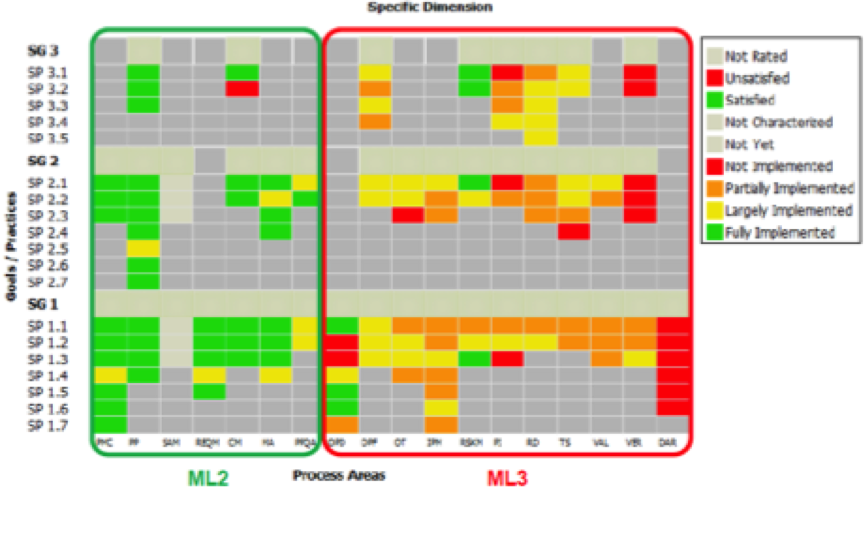
\includegraphics[width=0.86\textwidth]{thesis_goals}
%		\caption{SCAMPI results}
%		\label{fig:arch}
%	\end{center}
%\end{figure}

More specifically, the goals of this dissertation work are as follows: 

\begin{enumerate}[i]%for capital roman numbers.
	\item Analyze to what extent the SCRAIM tool supports the implementation (including the collection of evidences) of the specific practices of CMMI-DEV for maturiy levels 2 and 3 (ML2-3), and recommend relevant improvements to SCRAIM;
	\item Define rules to automatically assess the degree of fulfillment of CMMI-DEV ML2 practices by SCRAIM users, by analysing organizational project data and any other relevant evidences recorded in SCRAIM;
	\item Define questionnaires to assist the users in doing a manual assessment, for the practices  of CMMI-DEV ML2 that cannot be assessed automatically, ;
	\item Implement in SCRAIM rules and questionnaires defined in steps (ii) and (iii), for some process areas, including appropriate user interfaces to conduct assessments and visualize assessment results;
	\item Validate the electronic assessment approach in real world projects.
\end{enumerate}

The full-automated process is not yet feasible, so human intervention is still mandatory. With the use of SCRAIM, good practices will be followed and in the end the generated information will facilitate the decision making process. We can see many advantages of this innovation, and we believe that the application of this innovation will help reduce the costs and time of an evaluation using the SCAMPI method.

\section{Document structure} \label{sec:Structure}

This document is divided into six main chapters. The first and present chapter serves as an introduction where it is presented the context and motivation for this thesis as well as the goals and expected results to be delivered.

In chapter 2 it is made a problem analysis, giving insight about CMMI, SCAMPI and the tool to be used SCRAIM.

Chapter 3 presents the state of the art and related work regarding electronic assessment. It is described in detail the most used and most important tools that are currently being used in the appraisals.

In chapter 4 it is clarified the scope of the project and in chapter 5 it is made a description of the found solution.

Chapter 6 presents an example of usage and experimentation of the developed solution.

The final chapter sums up the document, presents the final conclusion and future work. 
			\chapter{Problem analysis} \label{chap:problem}

\section*{}

The evaluation for certification is one complex process, and requires many approaches, some acquired knowledge and some experience. To understand the problem and objectives of this dissertation, it is necessary to understand what is CMMI, in particular the SCAMPI \citep{SCAMPITeam2013} method and what is SCRAIM.

\section{CMMI}

\subsection{What is CMMI}

To understand better what is CMMI \citep{Development2010} we need to understand what is Capability model.

Capability Maturity Models contain essentially elements of effective processes, based on concepts developed by Crosby, Deming, Juran, and Humphrey.

The SEI (The Carnegie Mellon Software Engineering Institute that is a federally funded research and development center headquartered on the campus of Carnegie Mellon University in Pittsburgh, Pennsylvania, United States) adopted the process management premise, "the quality of a system or product is highly influenced by the quality of the process used to develop it and keep it" and defined CMMs that incorporated this premise.

\begin{figure}[h]
	\begin{center}
		\leavevmode
		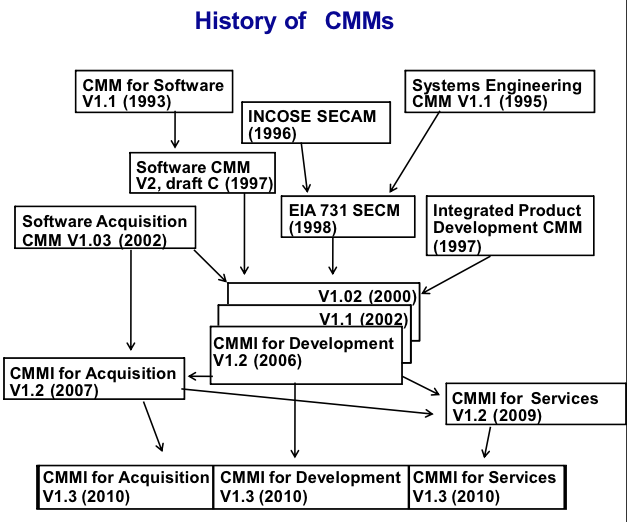
\includegraphics[width=0.86\textwidth]{CMMI_constelations}
		\caption{History of CMMs}
		\label{fig:historycmmi}
	\end{center}
\end{figure}

%referenciar a imagem no texto de alguma forma

CMMI stands for Capability Maturity Model Integration and is an evolution of CMM like shown in the Figure \ref{fig:historycmmi}.
It is a framework of best practices administered and sold by the Carnegie Mellon University, and for some business activities is required and mandatory like many DOD (United States Department of Defense) and U.S. Government contracts, especially in software development.


The CMMI model does not describe the processes themselves; it describes the characteristics of good processes, thus providing guidelines for companies developing or honing their own sets of processes.

Carnegie Mellon University says that CMMI can be used to guide an organization, a division and process improvement across projects. The CMMI processes and methodologies can be classified according to maturity levels.

Currently CMMI is on Version 1.3 and is registered in the United States Patent and Trademark Office by Carnegie Mellon University.

\subsection{CMMI models and process areas}
Best practices of CMMI are published in documents called models, each model addresses a different area of interest. The current version of CMMI, version 1.3, has three different areas of interest: development \citep{Chrissis2006}, acquisition and services.

These models are produced taking for base the CMMI framework that contains all the goals and practices used to produce the models that are part of CMMI constellations. The CMMI models contain 16 core process areas, they cover basic concepts fundamental to process improvement in any area of interest. 

The material in core process areas is almost the same for all constellations of CMMI, the rest of the material need to be adjusted to a specific area of interest, so the material wont be exactly the same.

\subsection{CMMI model framework}
CMMI framework is a basic structure that organizes and groups the CMMI components, elements of the current models, rules, methods for model generations, appraisal methods and training material, contains too process areas that will vary for each one of the CMMI areas that will be used. Process areas are the areas that cover the organization processes.

For the latest version of CMMI for Development (Version 1.3) there are 22 Process Areas, which represents the product aspects and the coverage for the organizational processes.


\subsection{CMMI representations}

CMMI is available in two representations: continuous and staged.

The continuous representation is represented by capability levels. Allows each organization to select the order of improvement that best meets their business objectives or those to which the organization assigns a high degree of risks. Enables comparisons across and among organizations on a process-area by process-area basis.


The staged representation is designed to provide a standard sequence of improvements, by maturity levels, each serving as foundation for the next. This representation results in a single rating (Maturity Level) that summarizes appraisal results and can serve as a basis for comparing the maturity of different projects and organizations.

\subsection{Maturity levels in CMMI for development}
\begin{figure}[h]
	\begin{center}
		\leavevmode
		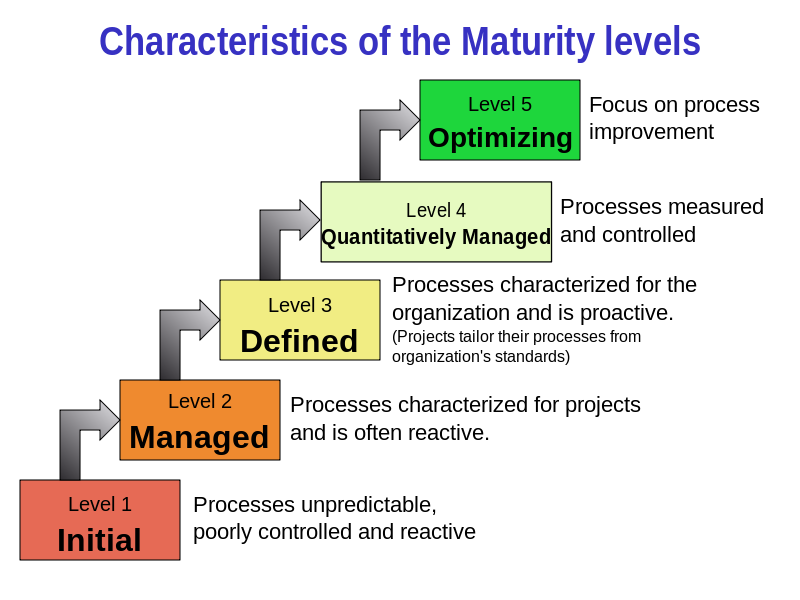
\includegraphics[width=0.86\textwidth]{Maturitylevels}
		\caption{CMMI maturity levels}
		\label{fig:maturitylevels}
	\end{center}
\end{figure}
Processes under the CMMI methodology are rated and grouped in maturity levels. There are five  maturity levels defined as: Initial, Managed, Defined, Quantitatively Managed, Optimizing. These maturity levels that are rated are presented and awarded for levels 2 through 5. The following process areas listed show us the maturity levels for CMMI for Development:

%\begin{itemize}
%	\item Maturity Level 2 - Managed
%	\begin{itemize}
%		\item CM - Configuration Management Measurement and Analysis
%		\item PMC - Project Monitoring and Control
%		\item PP - Project Planning
%		\item PPQA - Process and Product Quality Assurance
%		\item REQM - Requirements Management
%		\item SAM - Supplier Agreement Management
%
%	\end{itemize}
%	\item Maturity Level 3 - Defined
%	\begin{itemize}
%		\item DAR - Decision Analysis and Resolution
%		\item IPM - Integrated Project Management
%		\item OPD - Organizational Process Definition
%		\item OPF - Organizational Process Focus
%		\item OT - Organizational Training
%		\item PI - Product Integration
%		\item RD - Requirements Development
%		\item RSKM - Risk Management
%		\item TS - Technical Solution
%		\item VAL - Validation
%		\item VER – Verification	
%	\end{itemize}
%	\item Maturity Level 4 - Quantitatively Managed
%	\begin{itemize}
%		\item OPP - Organizational Process Performance
%		\item QPM - Quantitative Project Management		
%	\end{itemize}
%	\item Maturity Level 5 - Optimizing
%	\begin{itemize}
%	\item CAR - Causal Analysis and Resolution
%	\item OPM - Organizational Performance Management
%	\end{itemize}
%\end{itemize}

\subsection{Capability levels in CMMI for development}
A capability level is a well-defined evolutionary plateau describing the organization’s capability relative to a process area.

\subsection{Specific practices and generic practices}

\section{SCAMPI}
Organizations cannot be certified in CMMI, so there is something called appraisal and an organization is appraised.

In an appraisal the organization gets awarded a maturity level from one to five or a capability level achievement profile. As said before many organizations are required to get some kind of recognition and others find value measuring their progress and determining how well the processes adopted by the organization are compared to CMMI best practices, to meet contractual and customers requirements and to know which areas they can improve and appraisals are the right way to do it.

Appraisals using a CMMI model must comply with the requirements set out in the Appraisal Requirements for CMMI (ARC) document. There are three classes of appraisals, A, B and C. All of them compare the processes used in the organization to CMMI processes and best practices, that way is identified improvements to make. From all three classes of appraisals the most formal is class A and it is the only one that can output a level rating.

When an appraisal is done teams use a CMMI model and an ARC document. The results from the teams are used to plan improvements for the organization.

Statistics are made and updated every six months in a maturity profile since the release of CMMI show us that the median times to move from Level 1 to Level 2 is 5 months, and from that to Level 3 more 21 months.

\subsection{What is SCAMPI}
SCAMPI is the abbreviation for Standard CMMI Appraisal Method for Process Improvement and is an appraisal method that meets all the ARC requirements.
In SCAMPI appraisals there are three types of distinct classes: Class A, B and C appraisal methods. The most rigorous method and officially recognized as that is the Class A method and its the only method that can result in a benchmark quality rating. 
%SCAMPI B and C provide organizations improvements less formal than the class A, however still can identify improvements to be done.

Results SCAMPI appraisal can be published on the CMMI web site of SEI, if the organizations approves this. This appraisal supports ISO/IEC 15504, Software Process Improvement and Capability Determination (SPICE), a set of technical standards documents for the computer software development process and related business management functions.

The ARC Class A appraisals is normally conducted by SCAMPI A appraisal. The SCAMPI A Method Definition Document is where is defined rules to ensure the consistency of the appraisal ratings, so the same maturity rated in two companies means they are equal in methodologies and business processes.


\subsection{SCAMPI principles}
As said before the class A appraisal is the only full comprehensive appraisal method that involves an ARC class A method and uses CMMI models as reference models.

This appraisal will allow organizations to gain insight about their capability by identifying the strengths and weaknesses of its current processes, prioritize improvement plans, focus on those improvements, correcting weakness that will generate risks, derive capability rating as a maturity level rating and identify risks relative to capability and maturity determinations.

This appraisal follows these principals:
\begin{itemize}
	\item Start with a process reference model.
	\item Use a defined appraisal method.
	\item Involve senior management as an appraisal sponsor.
	\item Observe strict confidentiality and non-attribution.
	\item Approach the appraisal collaboratively. (When SCAMPI is used for Supplier Selection or Process Monitoring modes, it may not be
	possible to use a collaborative appraisal approach.)
	\item Focus on the sponsors business objectives
\end{itemize}

\subsection{The SCAMPI process}

The Method Definition Document is a document that describes SCAMPI appraisal method, this document sets the key elements of appraisal planning and the rules of conduct. It is also included in this document the level of process tailoring permitted, qualifications of the team members, evidence requirements, how to scope the appraisal and more.

There are essentially three phases in the process:
\begin{itemize}
	\item Phase I - Plan and Prepare for Appraisal 
	\item Phase II – Conduct Appraisal
	\item Phase III – Report Results
\end{itemize}

The following graphs shows us these phases where the last one includes the results report phase.

\begin{figure}[h]
	\begin{center}
		\leavevmode
		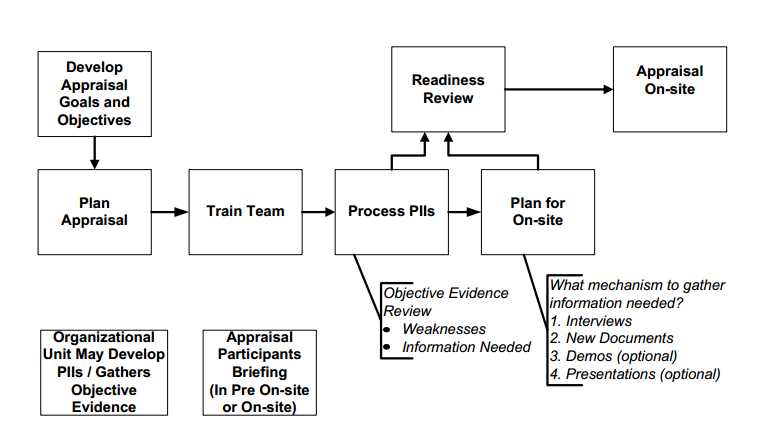
\includegraphics[width=0.86\textwidth]{appraisal_activies}
		\caption{Plan and Prepare for Appraisal Activities}
		\label{fig:plan_appraisal}
	\end{center}
\end{figure}


\begin{figure}[h]
	\begin{center}
		\leavevmode
		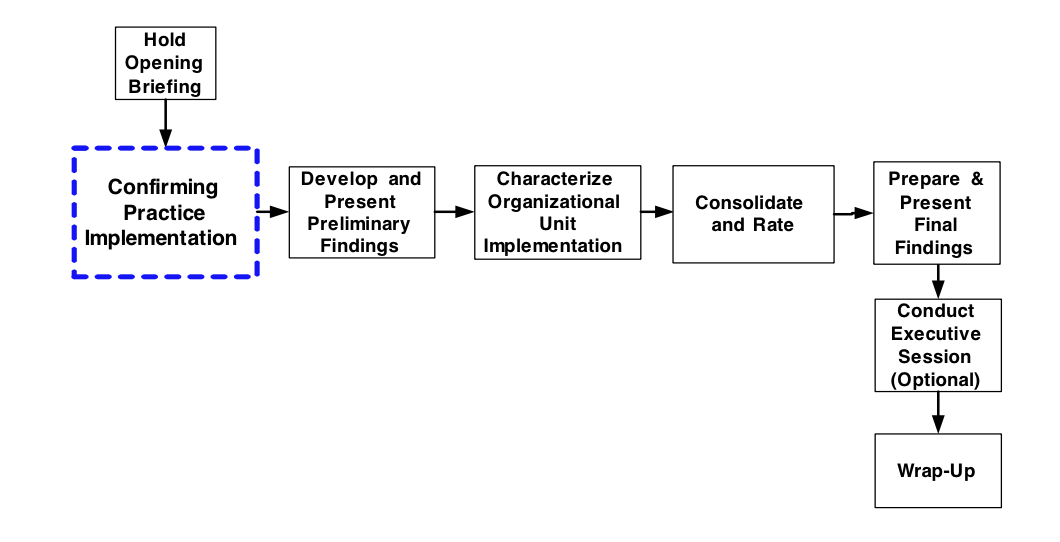
\includegraphics[width=0.86\textwidth]{phase2and3}
		\caption{Conduct Appraisal Activities}
		\label{fig:results_appraisal}
	\end{center}
\end{figure}

\subsection{Special terms}
There are some terms to consider with special meaning, Organizational Unit (OU), Organizational Scope, Subgroup, Basic Unit, Support Function, Objective Evidence, Instantiation, Database of Objective Evidence, Practice Characterization.

Organizational Unit is the subject of an appraisal. Can be deployed one or more processes that have a consistent process context, operates in a coherent set of business objectives and is typically part of a larger organization. In a small organization, this unit can be the whole organization.

Basic Unit stands for a set of interrelated and managed resources that delivers products or services to a customer and usually works like planned. The plan is documented and specifies the services or products delivered or implemented, the funds, the future work and the work that is currently being done.

A collection of basic unit and support functions that represent practices used within and organizational unit is the Organizational scope.


A Subgroup is a cluster of basic units that are shared between similar process implementations and a common sampling factor alternatives.

Support Function is an organizational group that for a certain and well defined set of activities needed by other parts of the organizations provides products and/or services.


Objective Evidence (OE) are indicators of the implementation or institutionalization of model practices. Verifying practice implementation is the review of Objective Evidence to determine whether a practice is implemented within a basic unit, support function, and/or organization. Can be of two types: artifacts or affirmations.
The artifacts are a tangible form of evidence indicative of work being done, which is both the main output of a practical model or a consequence of the implementation of a model of practice.
Affirmation is an oral or written statement confirming or support the implementation (or lack of implementation) in a practical model
provided by the practice performers, provide through an interactive forum in which the evaluation team has control over the
interaction.
In certain cases for some practices, documents are accepted as artifacts even if they are not the primary desired result of practical practice.

Instantiation is the implementation of a model practice used in its context in the organizational unit boundaries.

\subsection{Practice characterization}
Practices Implementation Indicators (PII) are a proof of  a correct implementation of a certain CMMI Practice. When a Practice is performed will leave a mark or evidence of that operation, for example that evidence can be a document produced while the practice is performed.

Appraisers look for an objective evidence in order to make an assessment. There are three types of indicators presented in the SCAMPI documentation.


\begin{table}[h]
	\centering
	\caption{Indicators Types}
\begin{tabular}{|p{2cm}|p{7cm}|p{4cm}|}
	\hline Indicator Type & Description & Examples\\
	\hline Direct artifacts & The tangible outputs resulting directly 
	from implementation of a specific or 
	generic practice. An integral part of 
	verifying practice implementation. May 
	be explicitly stated or implied by the 
	practice statement or associated 
	informative material. & Typical work products listed 
	in reference model practices 
	
	Target products of an 
	Establish and Maintain specific practice 
	
	Documents, deliverable 
	products, training materials, 
	etc. \\ 
	\hline Indirect artifacts & Artifacts that are a consequence of 
	performing a specific or generic practice 
	or that substantiate its implementation, 
	but which are not the purpose for which 
	the practice is performed. This indicator 
	type is especially useful when there may 
	be doubts about whether the intent of the 
	practice has been met (e.g., an artifact 
	exists but there is no indication of where 
	it came from, who worked to develop it, 
	or how it is used).  & Typical work products listed 
	in reference model practices 
	
	Meeting minutes, review 
	results, status reports, 
	presentations, etc. 
	
	Performance measures \\ 
	\hline Affirmations & Oral or written statements confirming or 
	supporting implementation (or lack of 
	implementation) of a specific or generic 
	practice. These statements are usually 
	provided by the implementers of the 
	practice and/or internal or external 
	customers, but may also include other 
	stakeholders (e.g., managers and 
	suppliers). &  Instruments 
	
	Interviews 
	
	Presentations, 
	demonstrations, etc.\\ 
	\hline 
\end{tabular}
\label{tab:Indicator}
\end{table}

 
\newpage
After the collection of an evidence and properly examined is made a characterization of the extent to which Model practices are implemented. The model practices are characterized as described in the next table.
\newline

\begin{table}[h]
	\centering
	\caption{Practice characterization table}
\begin{tabular}{|p{4cm}|p{9cm}|}
\hline
Fully Implemented (FI)   & Sufficient artifacts and/or affirmations are present and
judged to be adequate to demonstrate practice implementation, and
no weaknesses are noted.    \\
\hline
Largely Implemented (LI) & Sufficient artifacts and/or affirmations are present and
judged to be adequate to demonstrate practice implementation, and
one or more weaknesses are noted.  \\ 
\hline
Partially Implemented (PI) & Some or all data required are absent or judged to be
inadequate,
Some data are present to suggest some aspects of the practice are
implemented, and
one or more weaknesses are noted.


OR


Data supplied to the team (artifacts and/or affirmations) conflict –some data
indicate the practice is implemented and some data indicate the practice is
not implemented, and
one or more weaknesses are noted.\\
\hline
Not Implemented (NI) & Some or all data required are absent or judged to be
inadequate,
Data supplied does not support the conclusion that the practice is
implemented, and
one or more weaknesses are noted. \\
\hline
Not Yet (NY) & The basic unit or support function has not yet reached the stage in the
sequence of work, or point in time to have implemented the practice. \\
\hline
\end{tabular}
\label{tab:characterizations}
\end{table}





\subsection{Appraisal participants}
In an appraisal there are several participants with roles and responsibilities crucial to its success.

The Appraisal sponsor is responsible to sponsor the appraisal and owns the appraisal results and signs the Appraisal Disclosure Statement.

Middle managers are originally from the line or staff management positions and are interviewees and data providers and if they are participant they review preliminary findings.

Basic Unit leaders have leadership responsibilities for a project, service. They are too interviewees and data providers and if they are participant they review preliminary findings too.

Support Function as the past roles are interviewees and data providers, they are practitioners and review preliminary findings.

\subsection{Appraisal team}

The appraisal team is composed by two main Key Roles: Team Leader and Team Members.
Team Leader is the person who has the overall responsibility for the appraisal, is a SEI - Certified SCAMPI\citep{SCAMPITeam2013} leader appraisal and has experience and training, he signs too the final findings.
Team members are those who satisfy requirements of  experience and training to be part of the team and they assume one or more specific roles.

\subsection{Team leader responsibilities}

One of the key roles of the appraisal team is the team leader who has overall responsibility for the appraisal. He is also responsible for assign team roles for each member, ensuring that the planning activities are complete, that the SCAMPI process is being followed, scheduling monitoring and checking performance, facilitate team resolution in case of conflicts and impasses and reporting results to SEI.

\subsection{Team member responsibilities}
For each team member the team leader will assign a role that will ensure the proper function of the team and will facilitate the appraisal, those roles are the following:
\begin{itemize}
	\item Appraisal coordinator
	\subitem Responsible for handling on-site logistics. This position is also composed by more than one member for a multi-site appraisal.
	\item Librarian
	\subitem Documents are managed by this member and in the end of the appraisal they are returned.
	\item Timekeeper
	\subitem For each mini-team can be one Timekeeper and his main purpose is track team time and schedule constraints during interviews and other activities.
	\item Note takers
	\subitem For all PAs is responsible for taking notes during data gathering sessions.
	\item Appraisal team
	\subitem All the work is reviewed by members.
	\item Mini-teams
	\subitem Teams typically consist of two or three members and verify the implementation of reference model practices, reviewing objective evidence provided and identify weaknesses in the implementation. The practices at instantiation levels are characterized by its implementation extent. They have the power to request addition information if needed. 
\end{itemize}

\subsection{SCAMPI results}

The appraisal is completed after the collection and evaluation of objective evidence to support the implementation of practices.

Is set a Goal satisfaction that is based on extent to the practices associated with the goal implemented. The goal is rated if and only if all associated practices are characterized as largely implemented or fully implemented, and all the weaknesses associated with the defined goal don't have a significant impact on goal achievement.
With the of a program we can obtain a matrix as shown in the following image.
 
\begin{figure}[h]
	\begin{center}
		\leavevmode
		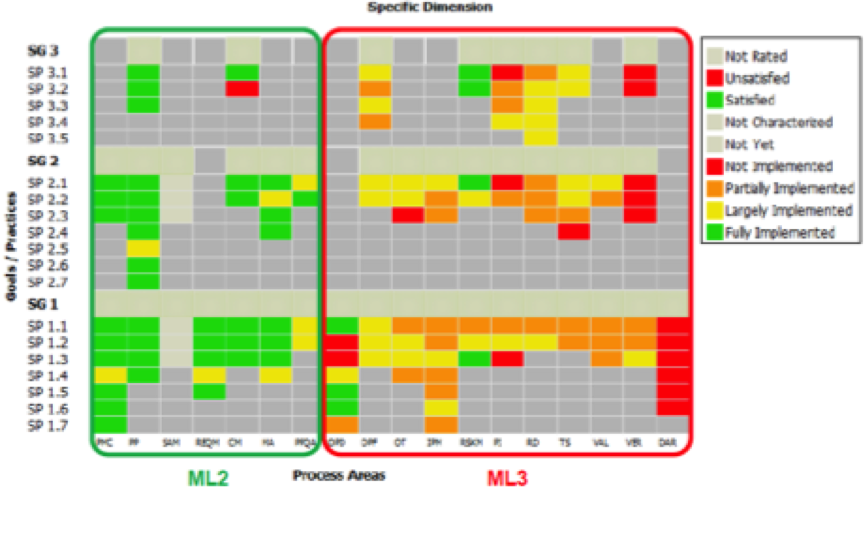
\includegraphics[width=0.86\textwidth]{thesis_goals}
		\caption{SCAMPI results}
		\label{fig:scampiresults}
	\end{center}
\end{figure}


When a given Goal is determined to be either Satisfied or not, then a Capability Level (for the continuous representation) can be derived and we can appraise.

\section{SCRAIM}

SCRAIM\citep{SCRAIM} is a project management tool based on advanced methodologies with intelligent decision support mechanisms. Also has some ready-made processes that facilitate a better management.

\subsection{Software as a service}

SCRAIM is a SaaS, which stands for Software-as-a-Service. Software-as-a-service (SaaS) emerges as an innovative
approach to deliver software applications based on cloud-computing
technology. \citep{Chou:2007:ANI:1359479.1359484}

This type of Software sometimes refered as simply hosted applications allows organizations and clients to access functionalities and all data stored on that platform everywhere, and it costs less than a typical licensed application. SaaS has many advantages compared to typical software, since is hosted remotely and accessed through Web they bypass the as server provisioning and software
installation as requirement, making software cheaper. Another advantage of this software type os that organizations don't need to perform and handle installation problems, updates and performing maintenance.

\begin{quote}
	``SaaS is one of the biggest technology trends to affect business
	applications in recent years.''~\cite{House2009}
\end{quote}
%Citar - SaaS is one of the biggest technology trends to affect business
%applications in recent years. (documento do SaaS)

\subsection{Methodologies and processes}
One of the reasons that can lead to a project failure is the lack of use of formal software development process, is also know that one of the success factors is the option of appropriate development process to the organizations projects.

\begin{figure}[h]
	\begin{center}
		\leavevmode
		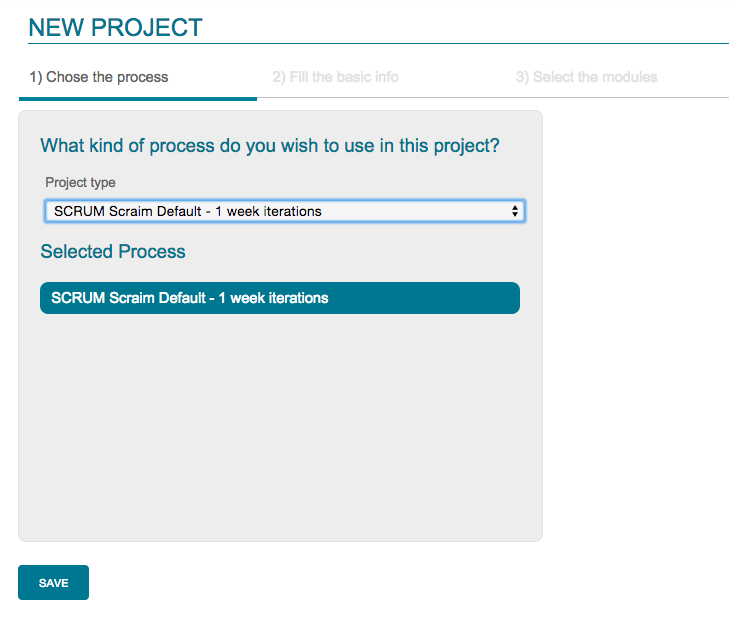
\includegraphics[width=0.5\textwidth]{ScraimProcessChoose}
		\caption{SCRAIM Process choose wizard}
		\label{fig:scraimrocesschoose}
	\end{center}
\end{figure}

SCRAIM is supported by the most advanced technologies like CMMI\citep{Development2010}, TSP and SixSigma\citep{SixSigmaWeb} to help organizations increase projects quality.
SCRAIM has a set of ready made processes like SCRUM\citep{Pries2011} and its possible to adapt to the specific needs of a project and save to use it later.

\subsection{Dashboard, issues, bug and time tracking}
This tool allow to track and organize projects tasks and team progress with a useful set of charts, is also part of this a set of features to facilitate team collaboration such as: wiki, forums, news and notification system.

Another feature if the scheduling of deliverables for each release of the organization project, with this its possible to know in real time what's being delivered, what's being schedule and who's in charge of each deliverable.

Risk Management is also supported by SCRAIM. This part of the software is designed for agile projects, giving the possibility to identify what can go wrong (risks), how to prevent that from happening (mitigation actions) and what to do if something happens (Impediments). 

In order to grant the quality of the project SCRAIM has a Test Management feature, this feature allows users to easily create and manage all the tests and track their results.

\begin{figure}[h]
	\begin{center}
		\leavevmode
		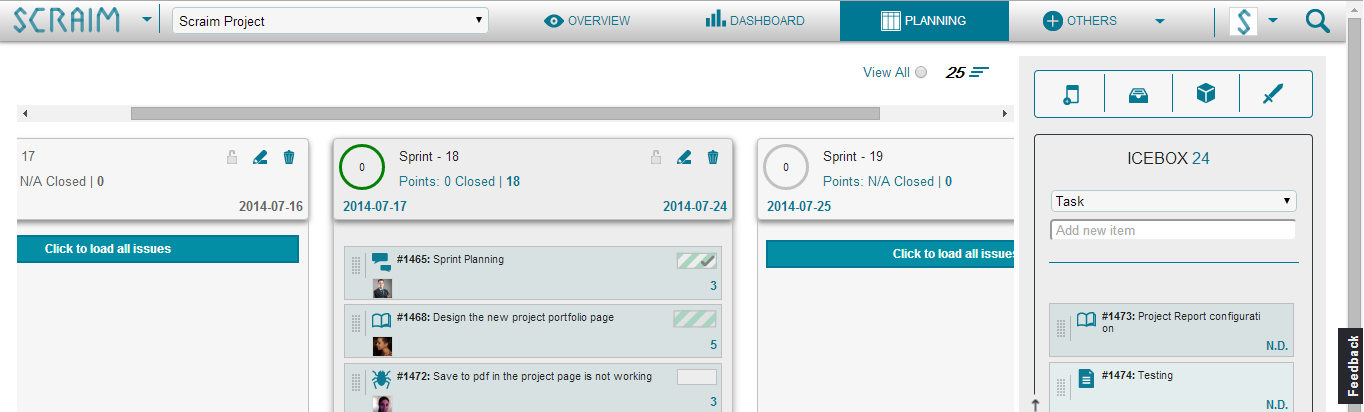
\includegraphics[width=0.86\textwidth]{ScraimPlanning}
		\caption{SCRAIM Planning View}
		\label{fig:scraimplanning}
	\end{center}
\end{figure}


\subsection{Documentation}

The project information is easily trackable cause SCRAIM allows  to manage files and documentation associated to each one of the projects and to attach external repositories in order to track the changes of source code.
			\chapter{State of the art analysis}\label{chap:chap3}

This chapter describes the related work associated with this problem, since this area is under explored the following tools are works that follow some analogue methodologies for other project processes like TSP, and some tools that are currently on the market and used for SCAMPI appraisals.

\section{CMMI assessment checklists and tools}
Leaders are recommended to identify the key business capabilities  by conducting a capability maturity assessment \citep{Hutchinson2014}, to determine and find what the organization need to build or strengthen the skills, designed to raise the company, business unit, or specific function to the next level. This tool appear as an online solution to make a lightweight assessment and is a free online assessment that make possible get and track an organization capability across eight key business functions based in a group of 31 questions.


\subsection{Assessment items}
In this tools each assessment item has a statement about a particular capability or several capabilities and a scale that allow to indicate the level of agreement with the statement, based on the organization performance. 

\begin{figure}[h]
	\begin{center}
		\leavevmode
		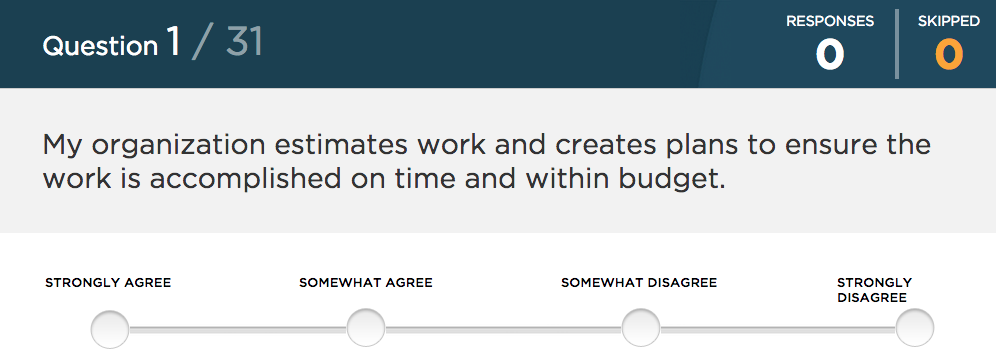
\includegraphics[width=0.75\textwidth]{cmmi_question}
		\caption{Assessment item question}
		\label{fig:cmmi_question}
	\end{center}
\end{figure}

The scale included in the assessment item also includes a descriptive information about the organization performance at both ends of the scale, visible on the example given below.

\begin{figure}[h]
	\begin{center}
		\leavevmode
		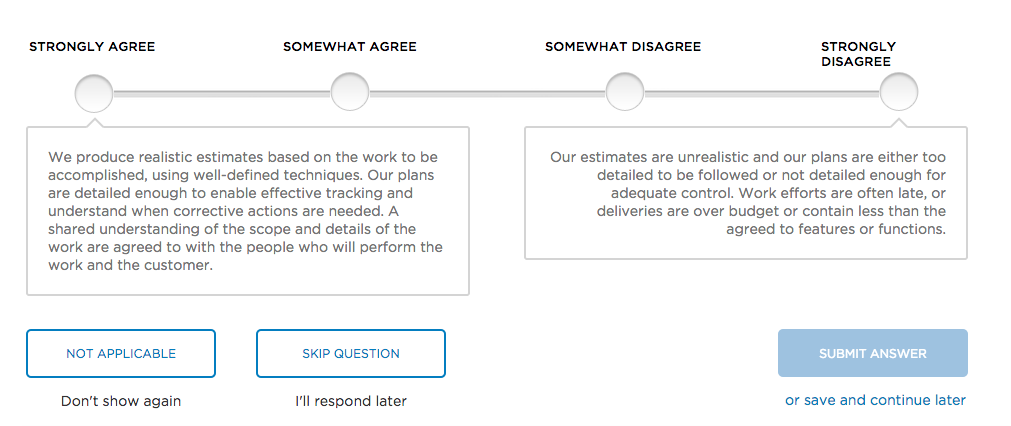
\includegraphics[width=0.86\textwidth]{respostascmmiassessment}
		\caption{Assessment item scale}
		\label{fig:assesment_answer}
	\end{center}
\end{figure}

These descriptions are given to the user with the intention of helping the most accurate positioning of the organization on the scale.

Organization term is defined by the user for purposes of  self-assessment. The evaluated scope is also by the user and can be the company, organizational unit, division, directorate, department or work group.

Its possible to skip a question in the list of items and comeback later to answer and there is an option named Not Applicable to exclude the question from the results, and this answer only should be choose if:
\begin{itemize}
	\item Actual question is related to an area outside of the organization scope.
	\item Its valid for the organization's but the  performance of the activities is not known.
	\item The user that is performing the assessment don't have sufficient expertise in the subject to understand the intent of the question.
\end{itemize}

The answers are editable before the submission of the assessment in a screen for a final review, is possible to save the current state and progress at any time and resume it later. Is only possible to submit and get an assessment if all questions are answered.

After answering all questions provided as requirement and those survey submitted will be show a high level snapshot of the organization  current capability states and will be included in each item some suggestions for developing the next steps.

\newpage

\begin{figure}[h]
	\begin{center}
		\leavevmode
		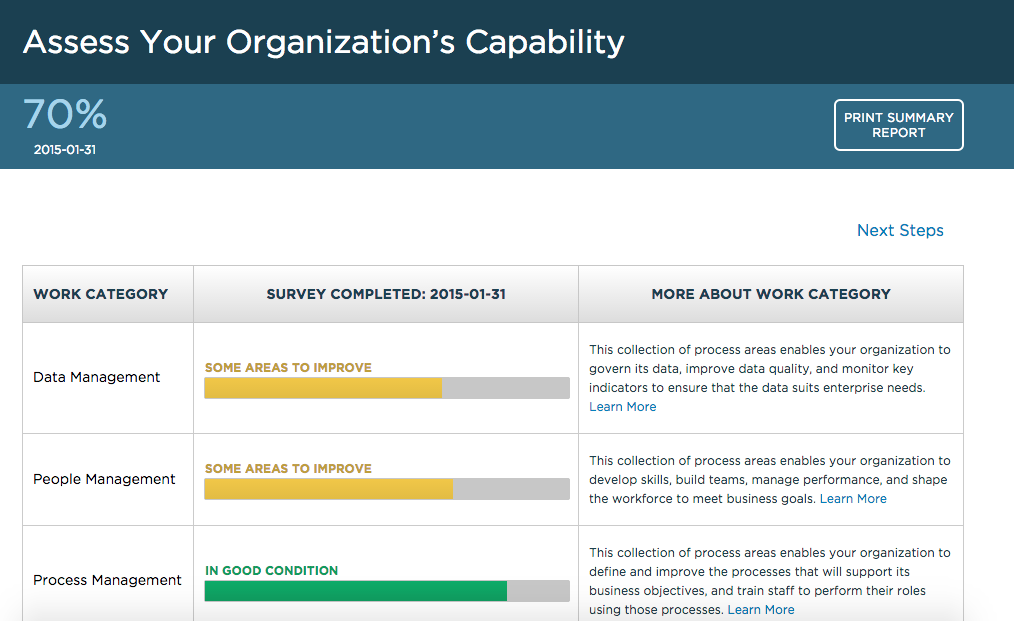
\includegraphics[width=0.96\textwidth]{resultcmmiassessment}
		\caption{Example of a result an assessment}
		\label{fig:assesment_result}
	\end{center}
\end{figure}


\section{PSP/TSP assessment checklists and tools}

PSP\citep{humphrey2005psp} is a process framework with the objective of guide developers to define their own processes, track and plan their work and manage the quality of the produced products.


\subsection{PSPchecker}

PSPChecker\citep{Pinto2010} is a tool that has the main objective of helping teachers to make decisions faster and help students to be able to achieve better results and understand PSP.

The PSPChecker was only made and planned for teachers as a support for evaluation and feedback it's suitable for students too depending on the type of teaching, that way they can improve their work. A short period of time is required to uses this tool and is currently only as a desktop application.


This desktop application has as main functionalities:
\begin{itemize}
	\item Automatic verification of checklists
	\subitem Each checklist item has different types of verification and as output if an item in the checklist is completely satisfied, it is shown the line in green otherwise red line is shown or given a special message on the screen.
	\item Custom processes
	\subitem The user when start the program can choose which items of the PSP process want to associate with this evaluation.
	\item Remote data importation
	\item Illustrative charts
	\subitem Charts that facilitate the perception of whats is wrong and well done to understand which points can be improved.
	\item Automation of support messages (use of knowledge acquired by specialists)
	\subitem Messages provided by specialist to understand the errors in a more complex level.
	\item Information Import/Export
	\begin{figure}[h]
		\begin{center}
			\leavevmode
			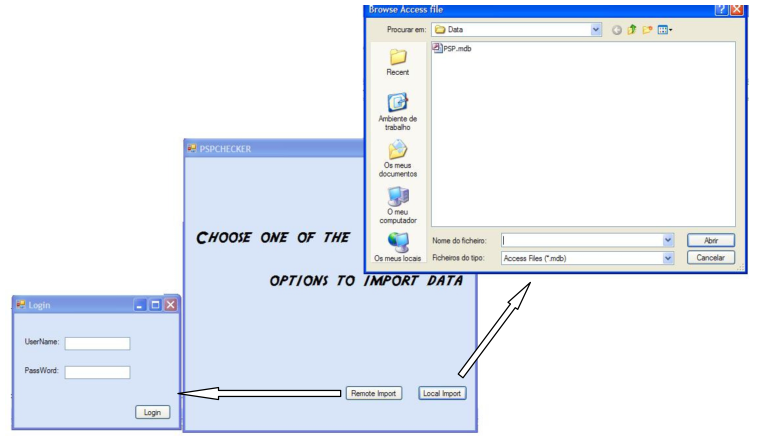
\includegraphics[width=0.63\textwidth]{PSPdataimport}
			\caption{Example of a data import for PSPChecker}
			\label{fig:PSPdataimport}
		\end{center}
	\end{figure}
	\item Modularity and scalability
\end{itemize}

\begin{figure}[h]
	\begin{center}
		\leavevmode
		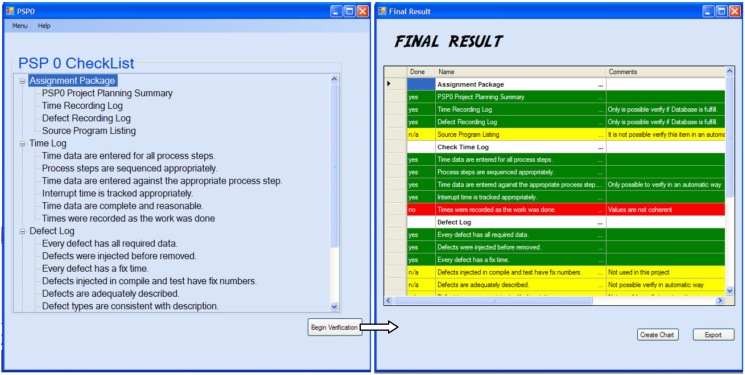
\includegraphics[width=0.8\textwidth]{PSPresult}
		\caption{Final results of PSPChecker}
		\label{fig:PSPdataimport}
	\end{center}
\end{figure}

In the Figure \ref{fig:PSPdataimport} is represented two of the last screens of PSPChecker. Is shown on the left side the checklist imported or chosen and on the right side the final screen, where we can generate charts and export the data.

\section{Appraisal Assistant}

The Software Quality Institute of the Griffith University\citep{SoftwareQuality2015} developed Appraisal Assistant. The Appraisal Assistant\citep{Appraisal2015} is a software application that supports the appraisal or assessment of process capability or organization maturity.

This tool follows consistent approaches with the requirements of ISO/IEC 15504(Information technology: Process assessment, and the Assessment Requirements for CMMI)\citep{ISOIEC} and it's distinguished from other tools by taking an evidence-driven approach to the record of evidences generated in an assessment.

SQI personnels have performed SCAMPI A and B appraisals and SPICE assessments with the help of Appraisal Assistant and have been using since the first beta release. The Beta release was used to examine relationships between ISO 15504-2 and SCAMPI appraisals

\begin{figure}[h]
	\begin{center}
		\leavevmode
		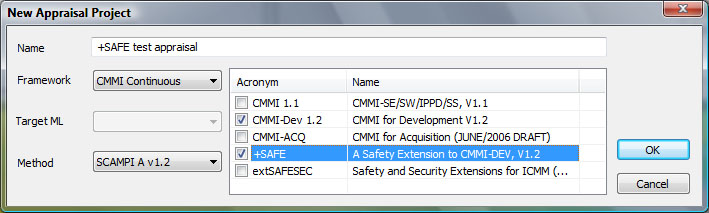
\includegraphics[width=0.8\textwidth]{newprojectsappraisal}
		\caption{Appraisal Assistant New Project Screen}
		\label{fig:newprojectsappraisal}
	\end{center}
\end{figure}

The Appraisal Assistant has many functionalities and can provide:
\begin{itemize}
	\item Support for multiple process models as: ISO/IEC 15504-5, ISO/IEC 15504-6 (FDIS), Automotive SPICE, CMMI®-DEV v.1.2, +SAFE, and CMMI® SE/SW/IPPD/SS V 1.1.
	\item User defined appraisal models.
	\item Multiple methods for performing appraisal / assessment.
	\item User defined assessment methods.
	\begin{figure}[h]
		\begin{center}
			\leavevmode
			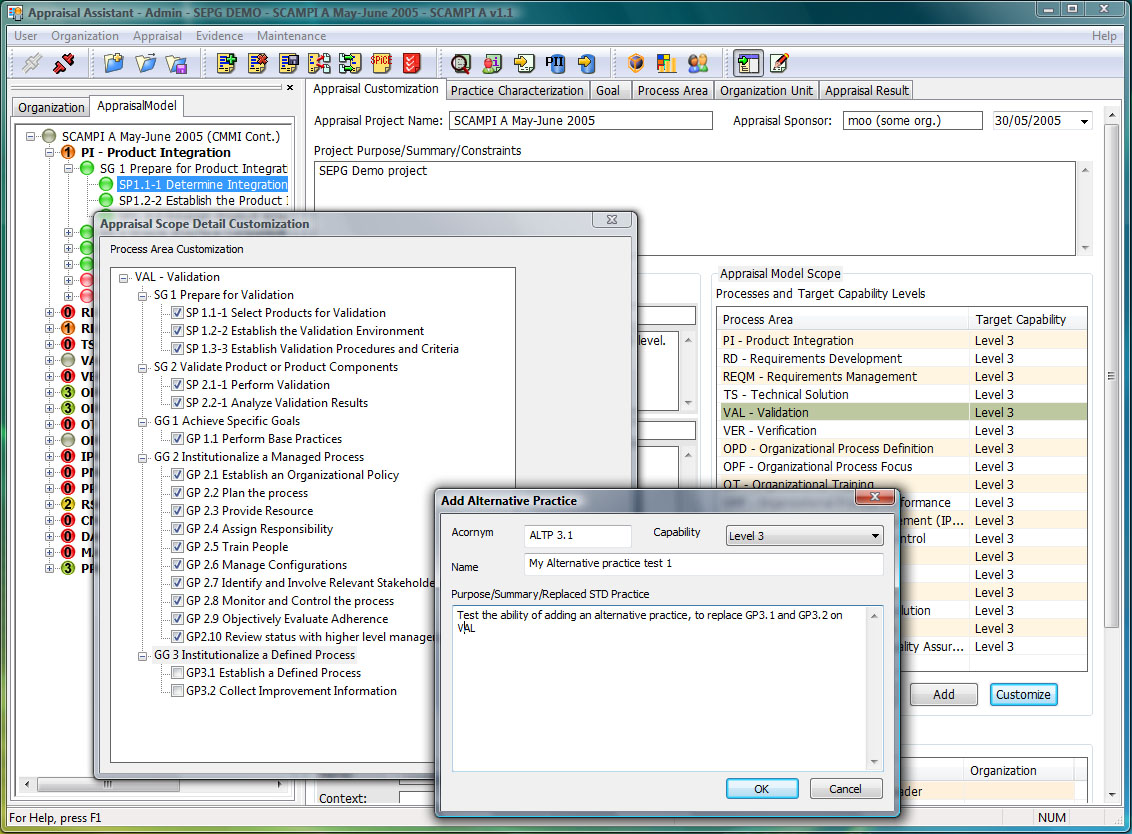
\includegraphics[width=0.6\textwidth]{cmmi_plan}
			\caption{Appraisal Scope Customization}
			\label{fig:cmmi_plan}
		\end{center}
	\end{figure}
	\item Conversion of results between frameworks
	\item Easy to split and consolidate evidence capture activities.
	\item Generate automatically reports as Appraisal Disclosure Statement, PIID, Assessment Record, Appraisal / Assessment Findings, Strength / Weakness summaries, Rating Profiles, and workload summaries.
	\item Model coverage and automatic reporting by collected evidence.
\end{itemize}


\begin{figure}[h]
	\begin{center}
		\leavevmode
		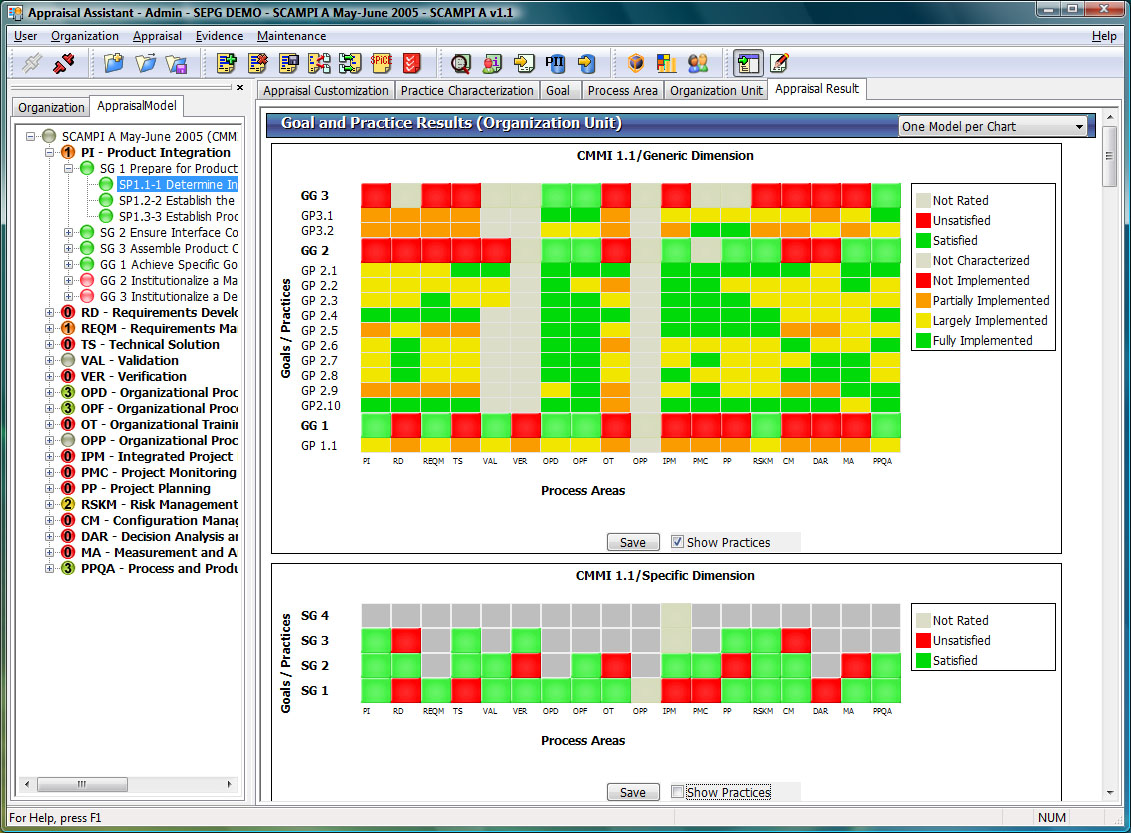
\includegraphics[width=0.6\textwidth]{cmmi_result}
		\caption{Appraisal Assistant Results}
		\label{fig:cmmi_result}
	\end{center}
\end{figure}

The Figure \ref{fig:cmmi_result} shows us an example of an appraisal result and output of the program after labeling all the process areas.
			\chapter{Solution perspectives}\label{chap:chap4}

\section{Envisioned approach}

The scheme represented by the Figure \ref{fig:envision}, resumes the envisioned approach.

\begin{figure}[h]
	\begin{center}
		\leavevmode
		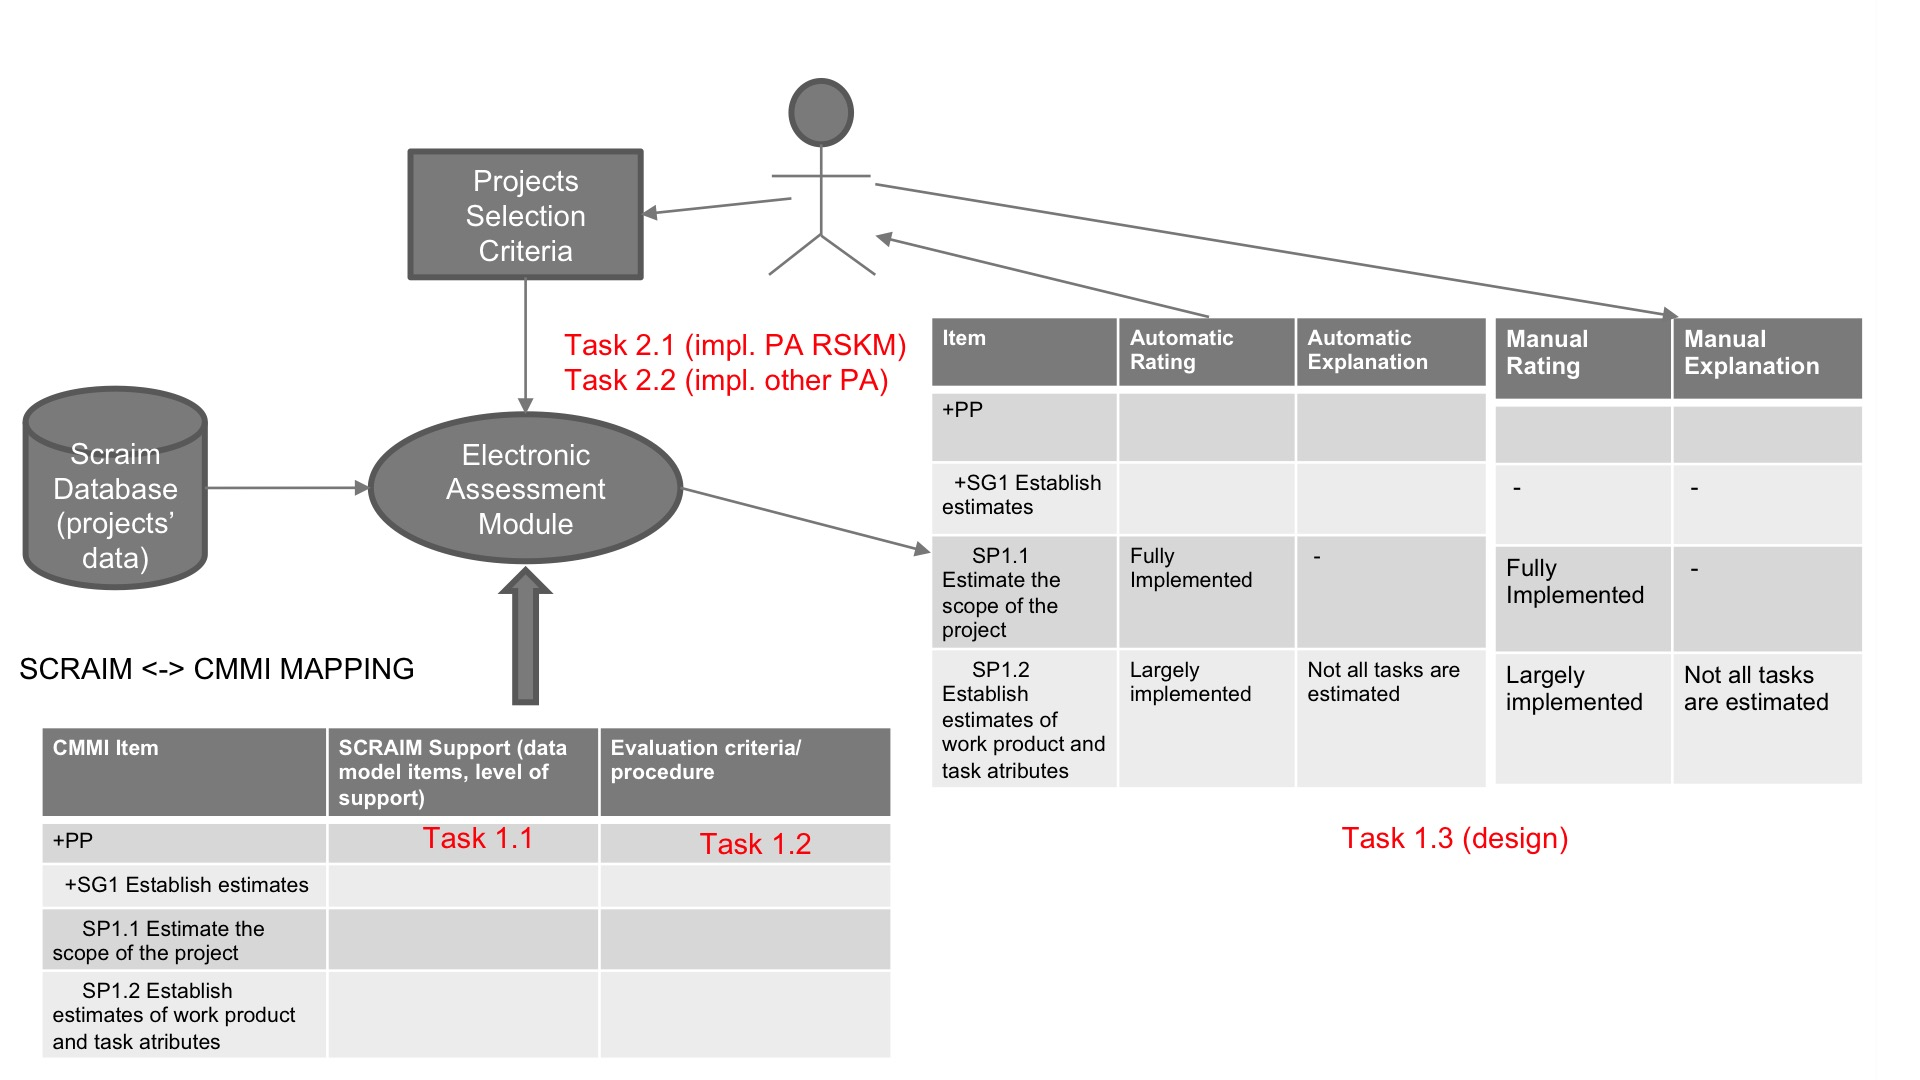
\includegraphics[width=1\textwidth]{envision}
		\caption{Envision approach scheme}
		\label{fig:envision}
	\end{center}
\end{figure}

The first step of this solution is to make a CMMI-SCRAIM mapping where it is going to be evaluated the data model items and the level of support available on SCRAIM and match them to CMMI best practices.

Then will be made the design of the module, where will be evaluated on a top level the data from SCRAIM database taking for base the previous mapping.

After completing these tasks will be evaluated the results obtained by this automatic rating and compared to manual ratings taking for base real projects selected from SCRAIM. 

For example in the Table \ref{tab:envision} its shown an automatic rating for the Project planning process area and the obtained explanation for that assessment. 


\begin{table}[h]
	\centering
	\caption{Automatic rating envision}
	\begin{tabular}{|p{6cm}|p{3cm}|p{3cm}|}
		\hline
		Item & Automatic Rating & Automatic Explanation\\
		\hline
		SG1 - Establish estimates&&\\
		SP 1.1 - Estimate scope of the project & Fully implemented & - \\
		SP 1.2 - Establish estimates of Work product and task attributes & Largely implemented & Not all tasks are estimated \\
		SP 1.3 - Define project lifecycle phases & Fully implemented & - \\
		SP 1.4 - Estimate effort and cost & Fully implemented & - \\
		\hline
		SG2 - Develop a project plan&&\\
		SP 2.1 - Establish the budget and schedule & Fully implemented & - \\
		SP 2.2 - Identify project risks & Partially implemented & Not all projects have risks identified \\
		SP 2.3 - Plan data Management & Fully implemented & - \\
		SP 2.4 - Plan the project's resources & Fully implemented & - \\
		SP 2.5 - Plan needed knowledge and skills & Fully implemented & - \\
		SP 2.6 - Plan stakeholder involvement & Not implemented & Not implemented \\
		SP 2.7 - Establish the project plan & Fully implemented & - \\
		\hline
		SG3 - Obtain commitment to the plan&&\\
		SP 3.1 - Review plans that affect the project & Fully implemented & - \\
		SP 3.2 - Reconcile work and resource levels & Fully implemented & - \\
		SP 3.3 - Obtain plan commitment & Largely implemented & Missing first meeting  \\
		\hline
	\end{tabular}
	\label{tab:envision}
\end{table}
\section{Work plan}

The work plan consists in four main tasks that are:
\begin{itemize}
	\item Conception - that contains the CMMI-SCRAIM mapping, definition of evaluation rules and user interface design.
	\item Implementation - consists in 6 iterations of one week each.
	\item Validation - analyze the results obtained by the module produced comparing to real assessments.
	\item Thesis and article writing
\end{itemize}

The Gantt of is presented on the Figure \ref{fig:workplan}.

\begin{figure}[h]
	\begin{center}
		\leavevmode
		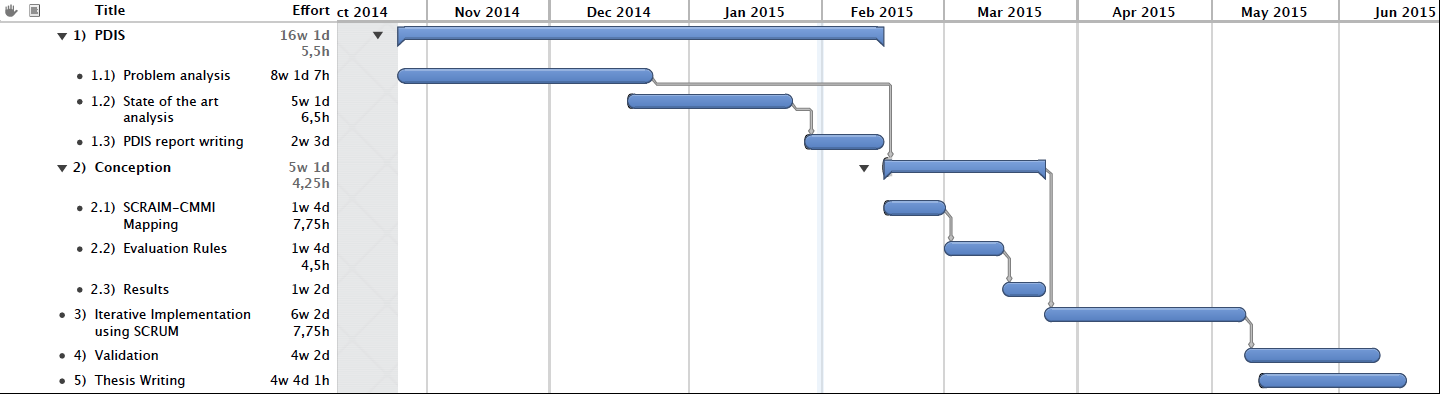
\includegraphics[width=1\textwidth]{workplan}
		\caption{Gantt Diagram}
		\label{fig:workplan}
	\end{center}
\end{figure}
			\chapter{Conclusions} \label{chap:concl} 

%The objective of this document is present and provide all the relevant information, the problem and the state-of-the-art.
%
%For that was explained in detail the concept of CMMI, SCAMPI and other important methodologies. The effort of SCAMPI evaluations
%
%The aim of this document is to provide the basis for the gathering of all relevant information and
%state-of-the-art relating to the area of long-term digital signatures. Another objective is to provide
%a solution to the problem that fulfills the goals described at the start. Both these objectives have
%been accomplished. 
			
			%%----------------------------------------
			%% Final materials
			%%----------------------------------------
			
			%% Bibliography
			%% Comment the next command if BibTeX file not used
			%% bibliography is in ``myrefs.bib''
			\PrintBib{myrefs}
			
			%% comment next 2 commands if numbered appendices are not used
			%\appendix
			%\chapter{Loren Ipsum} \label{ap1:loren}

			
			%% Index
			%% Uncomment next command if index is required
			%% don't forget to run ``makeindex pdis-en'' command
			%\PrintIndex
			
			\end{document}
